%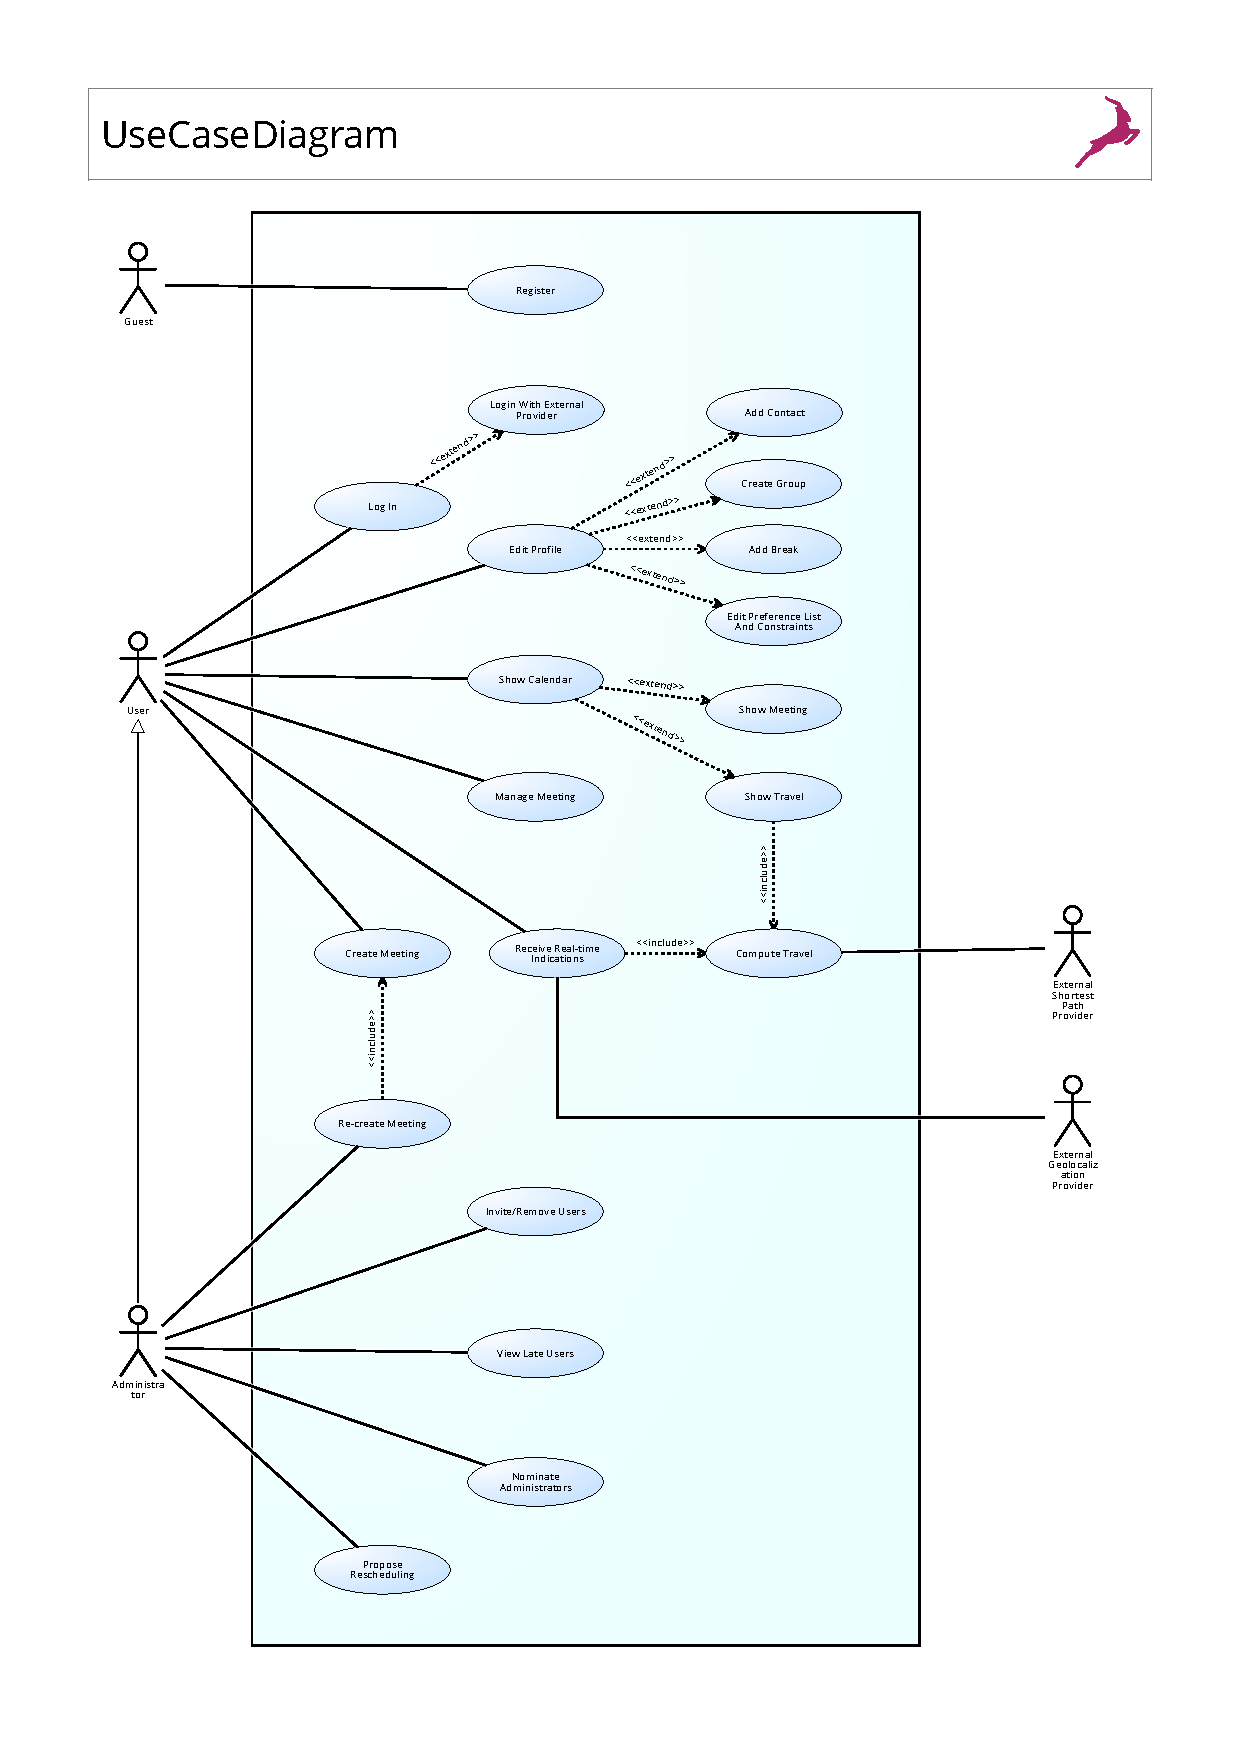
\includepdf[pages=-]{Pdf/UseCaseDiagram.pdf}

\begin{table}[H]
	\centering
	\caption{Use case description 1}
	\label{sect:uml:usecases:tab1}
	\def\arraystretch{1.5}
	\begin{tabular}{|p{7cm}|p{7cm}|}
		\hline
		\textbf{Actors}            & 		    \\ \hline
		\textbf{Goals}             &            \\ \hline
		\textbf{Input Conditions}  &            \\ \hline
		\textbf{Events Flow}       &            \\ \hline
		\textbf{Output Conditions} &            \\ \hline
		\textbf{Exceptions}        &            \\ \hline
	\end{tabular}
\end{table}

\begin{table}[H]
	\centering
	\caption{Use case description 1}
	\label{sect:uml:usecases:tab1}
	\def\arraystretch{1.5}
	\begin{tabular}{|p{7cm}|p{7cm}|}
		\hline
		\textbf{Actors}            & 		    \\ \hline
		\textbf{Goals}             &            \\ \hline
		\textbf{Input Conditions}  &            \\ \hline
		\textbf{Events Flow}       &            \\ \hline
		\textbf{Output Conditions} &            \\ \hline
		\textbf{Exceptions}        &            \\ \hline
	\end{tabular}
\end{table}

\begin{table}[H]
	\centering
	\caption{Use case description 1}
	\label{sect:uml:usecases:tab1}
	\def\arraystretch{1.5}
	\begin{tabular}{|p{7cm}|p{7cm}|}
		\hline
		\textbf{Actors}            & 		    \\ \hline
		\textbf{Goals}             &            \\ \hline
		\textbf{Input Conditions}  &            \\ \hline
		\textbf{Events Flow}       &            \\ \hline
		\textbf{Output Conditions} &            \\ \hline
		\textbf{Exceptions}        &            \\ \hline
	\end{tabular}
\end{table}